\documentclass[a4paper,12pt]{article}
\usepackage{graphicx}
\usepackage{float}
\usepackage[english,russian]{babel}

\title{1.1.4 Измерение интенсивности радиационного фона}
\author{Тимур Байдюсенов Б01-302}
\date{15.09.2023}

\begin{document}
\maketitle

\section{Аннотация}
В работе измеряется интенсивность радиационного фона. Данные фиксируются с помощью счётчика Гейгера-Мюллера(CTC-6). Исследуются ошибки результатов.

\section{Теоретические сведения}
Количество отсчётов в одном опыте подчиняется распределению Пуассона, т.к. регистрация частиц однородна по времени и каждая следующая не зависит от предыдущего.
Стандартная ошибка отдельного измерения находится по формуле:
\begin{equation}
\sigma=\sqrt{n}
\end{equation}
Значит результат измерений записывается так:
\begin{equation}
n_0=n\pm\sqrt{n}
\end{equation}
При $N$ измерениях среднее значение числа сосчитанных за одно измерение частиц равно:
\begin{equation}
\overline{n}=\frac{1}{N}\sum_{i=1}^{N} {n_i}
\end{equation}
Стандартную ошибку отдельного измерения можно оценить по формуле:
\begin{equation}
\sigma_{\mbox{отд}}=\sqrt{\frac{1}{N}\sum_{i=1}^{N}{(n_i-\overline{n})^2}}
\end{equation}
Ближе всего к значению $ \sigma_{\mbox{отд}} $ лежит величина $ \sqrt{\overline{n}} $, тогда:
\begin{equation}
\sigma_{\mbox{отд}} \approx \sqrt{{\overline{n}}}
\end{equation}
Как показывает теория вероятностей стандартная ошибка отклонения $\overline{n}$ от $n_0$ может быть определена так:
\begin{equation}
\sigma_{\overline{n}}=\frac{1}{N}\sqrt{\sum_{i=1}^N{(n_i-\overline{n})^2}}=\frac{\sigma_{\mbox{отд}}}{\sqrt{N}}
\end{equation}
Относительная ошибка отдельного измерения:
\begin{equation}
\varepsilon_{\mbox{отд}}=\frac{\sigma_{\mbox{отд}}}{n_i} \approx \frac{1}{\sqrt{n_i}}
\end{equation}
Аналогичным образом определяется относительная ошибка в определении среднего по всем измерениям значения $\overline{n}$:
\begin{equation}
\varepsilon_{\overline{n}}=\frac{\sigma_{\overline{n}}}{\overline{n}}=\frac{\sigma_{\mbox{отд}}}{\overline{n}\sqrt{N}}\approx\frac{1}{\sqrt{\overline{n}N}}
\end{equation}

\section{Оборудование}
\begin{figure}[H]
\centering
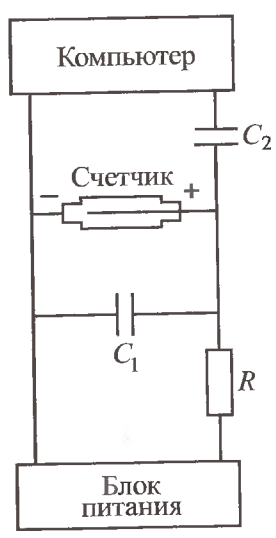
\includegraphics[width=0.25\textwidth]{счётчик}
\caption{Схема включения счетчика}
\end{figure}

Обнаружить космичекие лучи можно с помощью ионизации, которую они производят, используя счетчик Гейгера-Мюллера. Счетчик представляет собой наполненный газом сосуд с двумя электродами: металлическим цилиндром и нитью. Частицы космических лучей ионизируют газ, выбивая электроны из стенок сосуда и создавая лавину электронов: сталкиваясь с молекулами газа, выбивают из них электроны. Так, получается лавина электронов, в следствии чего, через счетчик увеличивается ток и регистрируется частица.

\section{Результаты измерений и обработка данных}

\begin{table}[H]
\centering
\caption{Число срабатываний счетчика за 20 с}
\begin{tabular}{|c|c|c|c|c|c|c|c|c|c|c|}
\hline
№ опыта : & 1 & 2 & 3 & 4 & 5 & 6 & 7 & 8 & 9 & 10 \\
\hline
0 : & 0 & 8 & 24 & 30 & 33 & 25 & 36 & 26 & 33 & 30 \\
10 : & 27 & 24 & 23 & 31 & 24 & 23 & 31 & 24 & 30 & 35 \\
20 : & 25 & 29 & 28 & 25 & 19 & 36 & 16 & 23 & 21 & 23 \\
30 : & 30 & 14 & 31 & 25 & 25 & 33 & 36 & 32 & 23 & 27 \\
40 : & 23 & 21 & 19 & 16 & 21 & 22 & 27 & 23 & 20 & 34 \\
50 : & 35 & 21 & 16 & 26 & 28 & 29 & 32 & 28 & 30 & 27 \\
60 : & 31 & 25 & 21 & 31 & 19 & 26 & 25 & 27 & 17 & 31 \\
70 : & 27 & 25 & 22 & 24 & 23 & 16 & 25 & 29 & 27 & 32 \\
80 : & 23 & 23 & 22 & 28 & 29 & 28 & 26 & 29 & 35 & 20 \\
90 : & 25 & 29 & 19 & 23 & 21 & 26 & 19 & 24 & 22 & 32 \\
100 : & 25 & 33 & 40 & 31 & 28 & 30 & 27 & 33 & 32 & 27 \\
110 : & 31 & 23 & 25 & 31 & 30 & 37 & 33 & 32 & 33 & 21 \\
120 : & 21 & 33 & 29 & 31 & 23 & 29 & 30 & 27 & 31 & 21 \\
130 : & 19 & 29 & 20 & 28 & 40 & 20 & 25 & 29 & 31 & 32 \\
140 : & 29 & 15 & 24 & 31 & 28 & 26 & 36 & 24 & 20 & 31 \\
150 : & 25 & 20 & 22 & 32 & 25 & 34 & 32 & 33 & 28 & 33 \\
160 : & 29 & 25 & 20 & 25 & 17 & 31 & 33 & 21 & 33 & 27 \\
170 : & 26 & 25 & 31 & 34 & 26 & 25 & 31 & 16 & 21 & 26 \\
180 : & 32 & 26 & 27 & 33 & 32 & 26 & 22 & 25 & 34 & 19 \\
190 : & 33 & 27 & 31 & 27 & 31 & 27 & 25 & 25 & 22 & 35 \\
\hline
\end{tabular}
\end{table}

\begin{table}[H]
\centering
\caption{Данные для построения гистограммы распределения числа срабатываний счетчика за 10 с} \label{10c}
\begin{tabular}{|c|c|c|c|c|c|}
\hline
Число импульсов $n_i$ & 4 & 5 & 6 & 7 & 8 \\
\hline
Число случаев & 2 & 6 & 6 & 6 & 22 \\
\hline
Доля случаев $w_n$ & 0.005 & 0.015 & 0.015 & 0.015 & 0.055 \\
\hline
\hline
Число импульсов $n_i$ & 9 & 10 & 11 & 12 & 13 \\
\hline
Число случаев & 22 & 30 & 44 & 37 & 47 \\
\hline
Доля случаев $w_n$ & 0.055 & 0.075 & 0.11 & 0.0925 & 0.1175 \\
\hline
\hline
Число импульсов $n_i$ & 14 & 15 & 16 & 17 & 18 \\
\hline
Число случаев & 54 & 30 & 22 & 25 & 19 \\
\hline
Доля случаев $w_n$ & 0.135 & 0.075 & 0.055 & 0.0625 & 0.0475 \\
\hline
\hline
Число импульсов $n_i$ & 19 & 20 & 21 & 22 & 23 \\
\hline
Число случаев & 8 & 7 & 5 & 2 & 1 \\
\hline
Доля случаев $w_n$ & 0.02 & 0.0175 & 0.0125 & 0.005 & 0.0025 \\
\hline
\hline
Число импульсов $n_i$ & 24 & 25 & 26 & 27 & 28\\
\hline
Число случаев & 0 & 1 & 0 & 0 & 1\\
\hline
Доля случаев $w_n$ & 0 & 0.0025 & 0 & 0 & 0.0025\\
\hline

\end{tabular}
\end{table}

\begin{table}[H]
\centering
\caption{Данные для построения гистограммы распределения числа срабатываний счетчика за 40 с} \label{40c}
\begin{tabular}{|c|c|c|c|c|c|}
\hline
Число импульсов $n_i$ & 42 & 43 & 44 & 45 & 46\\
\hline
Число случаев & 2 & 1 & 6 & 2 & 4 \\
\hline
Доля случаев $w_n$ & 0.02 & 0.01 & 0.06 & 0.02 & 0.04 \\
\hline
\hline
Число импульсов $n_i$ & 47 & 48 & 49 & 50 & 51\\
\hline
Число случаев & 4 & 4 & 5 & 7 & 6 \\
\hline
Доля случаев $w_n$ & 0.04 & 0.04 & 0.05 & 0.06 & 0.06 \\
\hline
\hline
Число импульсов $n_i$ & 52 & 53 & 54 & 55 & 56\\
\hline
Число случаев & 4 & 6 & 10 & 6 & 2 \\
\hline
Доля случаев $w_n$ & 0.04 & 0.06 & 0.1 & 0.06 & 0.02 \\
\hline
\hline
Число импульсов $n_i$ & 57 & 58 & 59 & 60 & 61\\
\hline
Число случаев & 4 & 7 & 2 & 1 & 3 \\
\hline
Доля случаев $w_n$ & 0.04 & 0.07 & 0.02 & 0.01 & 0.03 \\

\hline

\end{tabular}
\end{table}

Построим гистограммы 1, 2 на основе полученных данных. Они отображают распределение Пуассона и распределение Гаусса.

\begin{figure}[H]
\centering
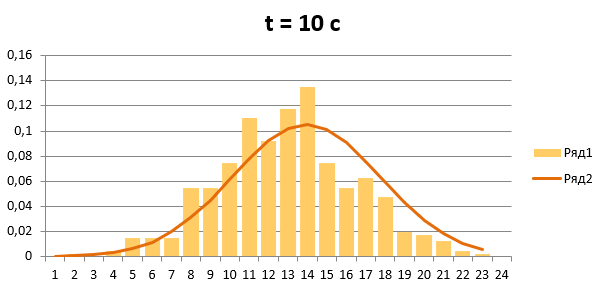
\includegraphics[width=1.1\textwidth]{график для 10}
\caption{Гистограмма для t = 10с}
\end{figure}
\begin{figure}[H]
\centering
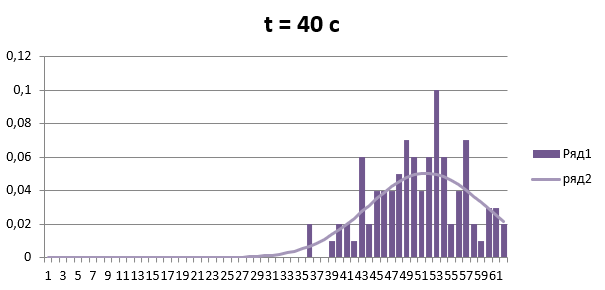
\includegraphics[width=1.1\textwidth]{график для 40}
\caption{Гистограмма для t = 40с}
\end{figure}

Определим среднее число частиц за 10 и 40 с:
\[\overline{n_{10}}=\frac{1}{N_{10}}\sum_{i=1}^{N_{10}} {n_i}=12.93\]
\[\overline{n_{40}}=\frac{1}{N_{40}}\sum_{i=1}^{N_{40}} {n_i}=51.72\]

Найдем среднеквадратичную ошибку отдельного измерения за 10 и 40 с по формуле:
\[\sigma_{\mbox{отд10}}=\sqrt{\frac{1}{N_{10}}\sum_{i=1}^{N_{10}}{(n_i-\overline{n_{10}})^2}}=3.79\]
\[\sigma_{\mbox{отд40}}=\sqrt{\frac{1}{N_{40}}\sum_{i=1}^{N_{40}}{(n_i-\overline{n_{40}})^2}}=7.88\]

Убедимся в справедливости формулы:
\[3.79\approx\sqrt{12.93}=3.60\]
\[7.88\approx\sqrt{51.72}=7.19\]

Найдем среднеквадратичное отклонение для средних значений по формуле:
\[\sigma_{\overline{n_{10}}}=\frac{\sigma_{\mbox{отд10}}}{\sqrt{N_{10}}}=0.19\]
\[\sigma_{\overline{n_{40}}}=\frac{\sigma_{\mbox{отд40}}}{\sqrt{N_{40}}}=0.79\]

Определим долю случаев для $t={\mbox{10 c}}$ и сравним с теоретическими оценками:
\begin{table}[H]
\centering
\begin{tabular}{|c|c|c|c|}
\hline
Ошибка & Число случаев & Доля случаев, \% & Теоретическая оценка \\
\hline
$\pm \sigma_{\text{отд10}}=\pm3.6$ & 264 & 66 & 68 \\
\hline
$\pm 2\sigma_{\text{отд10}}=\pm7.2$ & 379 & 94.75 & 95 \\
\hline
$\pm 3\sigma_{\text{отд10}}=\pm10.8$ & 395 & 98.75 & 99 \\
\hline
\end{tabular}
\end{table}

Определим долю случаев для $t={\mbox{40 c}}$ и сравним с теоретическими оценками:
\begin{table}[H]
\centering
\begin{tabular}{|c|c|c|c|}
\hline
Ошибка & Число случаев & Доля случаев, \% & Теоретическая оценка \\
\hline
$\pm \sigma_{\text{отд40}}=\pm7.2$ & 79 & 79 & 68 \\
\hline
$\pm 2\sigma_{\text{отд40}}=\pm14.4$ & 96 & 96 & 95 \\
\hline
$\pm 3\sigma_{\text{отд40}}=\pm21.6$ & 99 & 99 & 99 \\
\hline
\end{tabular}
\end{table}

Относительная ошибка:
\[\epsilon_{\overline{n_{10}}}=\frac{\sigma_{\overline{n_{10}}}}{\overline{n_{10}}}\approx1.5\%\]
\[\epsilon_{\overline{n_{40}}}=\frac{\sigma_{\overline{n_{40}}}}{\overline{n_{40}}}\approx1.5\%\]

Окончательный результат:
\[n_{10}=\overline{n_{10}}\pm\sigma_{\overline{n_{10}}}=12.93\pm0.19\]
\[n_{40}=\overline{n_{40}}\pm\sigma_{\overline{n_{40}}}=51.72\pm0.79\]

\section{Вывод}
В ходе выполнения работы познакомился с основными понятиями статистики: распределением Пуассона и распределением Гаусса. Удостоверился в возможности описания исследуемого процесса статистическими законами Пуассона и Гаусса. Определил среднее число регистрируемых космических лучей в секунду и определил погрешность результата.

\end{document}
